\newpage
\subsection{Caso d'uso UC10 - Visualizzazione API registrate}
\label{UC10}
\begin{figure}[ht]
	\centering
	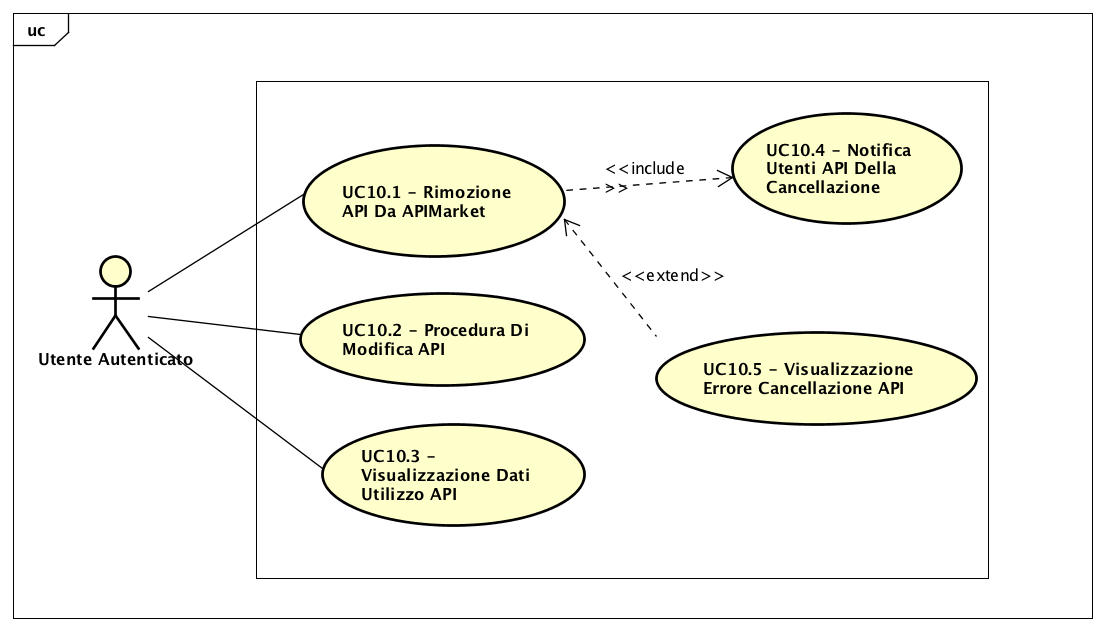
\includegraphics[scale=0.45]{UML/UC10.png}
	\caption{UC10: Visualizzazione API registrate}
\end{figure}

\begin{longtable}{ l | p{11cm}}
	\hline
	\rowcolor{Gray}
	\multicolumn{2}{c}{UC10 - Visualizzazione API registrate}\\
	\hline
	
	 \textbf{Attori} & Utente autenticato  \\
	\textbf{Descrizione} & L'attore può visualizzare la schermata relativa alle API da lui registrate \\
	\textbf{Pre-Condizioni} & L'attore seleziona il link per visualizzare le API registrate  \\
	\textbf{Post-Condizioni} & L'attore visualizza la pagina relativa alle API da lui registrate\\
	\textbf{Scenario Principale} & 
	\begin{enumerate*}[label=(\arabic*.),itemjoin={\newline}]
		\item L'attore visualizza il numero di API registrate (UC10.1)
		\item L'attore visualizza la lista di API registrate (UC10.2)
	\end{enumerate*}\\
	\textbf{Scenari Alternativi} & 
	\begin{enumerate*}[label=(\arabic*.),itemjoin={\newline}]
		\item L'attore può visualizzare i dati relativi a una singola API (UC7)
	\end{enumerate*}\\
\end{longtable}


\subsubsection{Caso d'uso UC10.1: Visualizzazione numero API registrate}
\label{UC10_1}

\begin{minipage}{\linewidth}
	\begin{tabular}{ l | p{11cm}}
		\hline
		\rowcolor{Gray}
		\multicolumn{2}{c}{UC10.1 - Visualizzazione numero API registrate} \\
		\hline
		\textbf{Attori} & Utente autenticato \\
		\textbf{Descrizione} & L'attore visualizza il numero di API da lui registrate nella schermata relativa\\
		\textbf{Pre-Condizioni} & L'attore si trova nel menù relativo alle API da lui registrate\\
		\textbf{Post-Condizioni} & L'attore visualizza il numero di API registrate \\
		\textbf{Scenario Principale} & 
		\begin{enumerate*}[label=(\arabic*.),itemjoin={\newline}]
			\item L'attore può visualizzare il numero di API da lui registrate nella piattaforma
		\end{enumerate*}\\
	\end{tabular}
\end{minipage}

\subsubsection{Caso d'uso UC10.2: Visualizzazione lista API registrate}
\label{UC10_2}

\begin{minipage}{\linewidth}
	\begin{tabular}{ l | p{11cm}}
		\hline
		\rowcolor{Gray}
		\multicolumn{2}{c}{UC10.2 - Visualizzazione lista API registrate} \\
		\hline
		\textbf{Attori} & Utente autenticato \\
		\textbf{Descrizione} & L'attore visualizza la lista di API da lui registrate nella schermata relativa\\
		\textbf{Pre-Condizioni} & L'attore si trova nel menù relativo alle API da lui registrate\\
		\textbf{Post-Condizioni} & L'attore visualizza la lista di API registrate \\
		\textbf{Scenario Principale} & 
		\begin{enumerate*}[label=(\arabic*.),itemjoin={\newline}]
			\item L'attore visualizza il nome dell'API (10.2.1)
			\item L'attore visualizza il link alla pagina dell'API (10.2.2)
			\item L'attore visualizza il numero di licenze attive (10.2.3)
			\item L'attore visualizza un pulsante per la modifica dell'API selezionata (10.2.4)
			\item L'attore visualizza un pulsante per l'eliminazione (10.2.5)
		\end{enumerate*}\\
	\end{tabular}
\end{minipage}

\paragraph{Caso d'uso UC10.2.1: Visualizzazione nome API}
\label{UC10_2_1}

\begin{minipage}{\linewidth}
	\begin{tabular}{ l | p{11cm}}
		\hline
		\rowcolor{Gray}
		\multicolumn{2}{c}{UC10.2.1 - Visualizzazione nome API} \\
		\hline
		\textbf{Attori} & Utente autenticato \\
		\textbf{Descrizione} & L'attore visualizza il nome dell'API\\
		\textbf{Pre-Condizioni} & L'attore visualizza la lista API nel menù relativo alle API da lui registrate\\
		\textbf{Post-Condizioni} & L'attore visualizza il nome dell'API nella lista \\
		\textbf{Scenario Principale} & 
		\begin{enumerate*}[label=(\arabic*.),itemjoin={\newline}]
			\item L'attore può visualizzare il nome dell'API
		\end{enumerate*}\\
	\end{tabular}
\end{minipage}

\paragraph{Caso d'uso UC10.2.2: Visualizzazione link API}
\label{UC10_2_2}

\begin{minipage}{\linewidth}
	\begin{tabular}{ l | p{11cm}}
		\hline
		\rowcolor{Gray}
		\multicolumn{2}{c}{UC10.2.2 - Visualizzazione link API} \\
		\hline
		\textbf{Attori} & Utente autenticato \\
		\textbf{Descrizione} & L'attore visualizza il link dell'API\\
		\textbf{Pre-Condizioni} & L'attore visualizza la lista API nel menù relativo alle API da lui registrate\\
		\textbf{Post-Condizioni} & L'attore visualizza il link dell'API nella lista \\
		\textbf{Scenario Principale} & 
		\begin{enumerate*}[label=(\arabic*.),itemjoin={\newline}]
			\item L'attore può visualizzare il link dell'API
		\end{enumerate*}\\
	\end{tabular}
\end{minipage}

\paragraph{Caso d'uso UC10.2.3: Visualizzazione numero licenze attive}
\label{UC10_2_3}

\begin{minipage}{\linewidth}
	\begin{tabular}{ l | p{11cm}}
		\hline
		\rowcolor{Gray}
		\multicolumn{2}{c}{UC10.2.3 - Visualizzazione numero licenze attive} \\
		\hline
		\textbf{Attori} & Utente autenticato \\
		\textbf{Descrizione} & L'attore visualizza il numero di licenze attive per ogni voce della lista\\
		\textbf{Pre-Condizioni} & L'attore visualizza la lista API nel menù relativo alle API da lui registrate\\
		\textbf{Post-Condizioni} & L'attore visualizza il numero delle API vendute e attualmente attive \\
		\textbf{Scenario Principale} & 
		\begin{enumerate*}[label=(\arabic*.),itemjoin={\newline}]
			\item L'attore può visualizzare il numero delle API vendute e attualmente attive
		\end{enumerate*}\\
	\end{tabular}
\end{minipage}

\paragraph{Caso d'uso UC10.2.4: Modifica API registrata}
\label{UC10_2_4}

\begin{minipage}{\linewidth}
	\begin{tabular}{ l | p{11cm}}
		\hline
		\rowcolor{Gray}
		\multicolumn{2}{c}{UC10.2.4 - Modifica API registrata} \\
		\hline
		\textbf{Attori} & Utente autenticato \\
		\textbf{Descrizione} & L'attore visualizza il menù di modifica per l'API selezionata\\
		\textbf{Pre-Condizioni} & L'attore preme il pulsante modifica per un API, nel menù relativo alle API da lui registrate\\
		\textbf{Post-Condizioni} & L'attore ha modificato un API registrata \\
		\textbf{Scenario Principale} & 
		\begin{enumerate*}[label=(\arabic*.),itemjoin={\newline}]
			\item L'attore può modificare il nome dell'API (UC10.2.4.1)
			\item L'attore può modificare la descrizione dell'API (UC10.2.4.2)
			\item L'attore può modificare i tag dell'API (UC10.2.4.3)
			\item L'attore può modificare l'interfaccia pubblica dell'API (UC10.2.4.4)
			\item L'attore può modificare il link esterno alla documentazione (UC10.2.4.5)
			\item L'attore può modificare il file di documentazione caricato  (UC10.2.4.6)
			\item L'attore può modificare il prezzo base per l'API (UC10.2.4.7)
			\item L'attore può confermare i dati modificati e continuare con l'operazione (UC10.2.4.8)
		\end{enumerate*}\\
		\textbf{Scenari Alternativi} & 
		\begin{enumerate*}[label=(\arabic*.),itemjoin={\newline}]
			\item L'attore riceve un errore relativo ai dati modificati, e la richiesta non viene completata (UC10.2.4.9)
		\end{enumerate*}\\
	\end{tabular}
\end{minipage}

\subparagraph{Caso d'uso UC10.2.4.1: Modifica nome API registrata}
\label{UC10_2_4_1}

\begin{minipage}{\linewidth}
	\begin{tabular}{ l | p{11cm}}
		\hline
		\rowcolor{Gray}
		\multicolumn{2}{c}{UC10.2.4.1 - Modifica nome API registrata} \\
		\hline
		\textbf{Attori} & Utente autenticato \\
		\textbf{Descrizione} & L'attore modifica il nome relativo ad una propria API\\
		\textbf{Pre-Condizioni} & L'attore si trova nella schermata per la modifica di un'API da lui registrata\\
		\textbf{Post-Condizioni} & L'attore ha modificato il nome dell'API selezionata \\
		\textbf{Scenario Principale} & 
		\begin{enumerate*}[label=(\arabic*.),itemjoin={\newline}]
			\item L'attore può modificare il nome dell'API
		\end{enumerate*}\\
	\end{tabular}
\end{minipage}

\subparagraph{Caso d'uso UC10.2.4.2: Modifica descrizione API registrata}
\label{UC10_2_4_2}

\begin{minipage}{\linewidth}
	\begin{tabular}{ l | p{11cm}}
		\hline
		\rowcolor{Gray}
		\multicolumn{2}{c}{UC10.2.4.2 - Modifica descrizione API registrata} \\
		\hline
		\textbf{Attori} & Utente autenticato \\
		\textbf{Descrizione} & L'attore modifica la descrizione relativa ad una propria API\\
		\textbf{Pre-Condizioni} & L'attore si trova nella schermata per la modifica di un'API da lui registrata\\
		\textbf{Post-Condizioni} & L'attore ha modificato la descrizione dell'API selezionata \\
		\textbf{Scenario Principale} & 
		\begin{enumerate*}[label=(\arabic*.),itemjoin={\newline}]
			\item L'attore può modificare la descrizione dell'API
		\end{enumerate*}\\
	\end{tabular}
\end{minipage}

\subparagraph{Caso d'uso UC10.2.4.3: Modifica tag API registrata}
\label{UC10_2_4_3}

\begin{minipage}{\linewidth}
	\begin{tabular}{ l | p{11cm}}
		\hline
		\rowcolor{Gray}
		\multicolumn{2}{c}{UC10.2.4.3 - Modifica tag API registrata} \\
		\hline
		\textbf{Attori} & Utente autenticato \\
		\textbf{Descrizione} & L'attore modifica i tag relativi ad una propria API\\
		\textbf{Pre-Condizioni} & L'attore si trova nella schermata per la modifica di un'API da lui registrata\\
		\textbf{Post-Condizioni} & L'attore ha modificato i tag dell'API selezionata \\
		\textbf{Scenario Principale} & 
		\begin{enumerate*}[label=(\arabic*.),itemjoin={\newline}]
			\item L'attore può modificare i tag dell'API
		\end{enumerate*}\\
	\end{tabular}
\end{minipage}

\subparagraph{Caso d'uso UC10.2.4.4: Modifica interfaccia API registrata}
\label{UC10_2_4_4}

\begin{minipage}{\linewidth}
	\begin{tabular}{ l | p{11cm}}
		\hline
		\rowcolor{Gray}
		\multicolumn{2}{c}{UC10.2.4.4 - Modifica interfaccia API registrata} \\
		\hline
		\textbf{Attori} & Utente autenticato \\
		\textbf{Descrizione} & L'attore modifica l'interfaccia pubblica relativa ad una propria API\\
		\textbf{Pre-Condizioni} & L'attore si trova nella schermata per la modifica di un'API da lui registrata\\
		\textbf{Post-Condizioni} & L'attore ha modificato l'interfaccia pubblica dell'API selezionata \\
		\textbf{Scenario Principale} & 
		\begin{enumerate*}[label=(\arabic*.),itemjoin={\newline}]
			\item L'attore può modificare l'interfaccia pubblica dell'API
		\end{enumerate*}\\
	\end{tabular}
\end{minipage}

\subparagraph{Caso d'uso UC10.2.4.5: Modifica link documentazione API registrata}
\label{UC10_2_4_5}

\begin{minipage}{\linewidth}
	\begin{tabular}{ l | p{11cm}}
		\hline
		\rowcolor{Gray}
		\multicolumn{2}{c}{UC10.2.4.5 - Modifica link documentazione API registrata} \\
		\hline
		\textbf{Attori} & Utente autenticato \\
		\textbf{Descrizione} & L'attore modifica il link di documentazione esterna relativo ad una propria API\\
		\textbf{Pre-Condizioni} & L'attore si trova nella schermata per la modifica di un'API da lui registrata\\
		\textbf{Post-Condizioni} & L'attore ha modificato il link di documentazione esterna dell'API selezionata \\
		\textbf{Scenario Principale} & 
		\begin{enumerate*}[label=(\arabic*.),itemjoin={\newline}]
			\item L'attore può modificare il link di documentazione esterna dell'API
		\end{enumerate*}\\
	\end{tabular}
\end{minipage}

\subparagraph{Caso d'uso UC10.2.4.6: Modifica file documentazione API registrata}
\label{UC10_2_4_6}

\begin{minipage}{\linewidth}
	\begin{tabular}{ l | p{11cm}}
		\hline
		\rowcolor{Gray}
		\multicolumn{2}{c}{UC10.2.4.6 - Modifica file documentazione API registrata} \\
		\hline
		\textbf{Attori} & Utente autenticato \\
		\textbf{Descrizione} & L'attore modifica il file di documentazione relativo ad una propria API\\
		\textbf{Pre-Condizioni} & L'attore si trova nella schermata per la modifica di un'API da lui registrata\\
		\textbf{Post-Condizioni} & L'attore ha modificato il file di documentazione dell'API selezionata \\
		\textbf{Scenario Principale} & 
		\begin{enumerate*}[label=(\arabic*.),itemjoin={\newline}]
			\item L'attore può selezionare un nuovo file dalle sue cartelle personali, che verrà caricato alla conferma
		\end{enumerate*}\\
		\textbf{Scenario Principale} & 
		\begin{enumerate*}[label=(\arabic*.),itemjoin={\newline}]
			\item Il file selezionato è di un formato non conforme e l'operazione non avviene
		\end{enumerate*}\\
	\end{tabular}
\end{minipage}

\subparagraph{Caso d'uso UC10.2.4.7: Modifica prezzo API registrata}
\label{UC10_2_4_7}

\begin{minipage}{\linewidth}
	\begin{tabular}{ l | p{11cm}}
		\hline
		\rowcolor{Gray}
		\multicolumn{2}{c}{UC10.2.4.7 - Modifica prezzo API registrata} \\
		\hline
		\textbf{Attori} & Utente autenticato \\
		\textbf{Descrizione} & L'attore modifica il prezzo base relativo ad una propria API\\
		\textbf{Pre-Condizioni} & L'attore si trova nella schermata per la modifica di un'API da lui registrata\\
		\textbf{Post-Condizioni} & L'attore ha modificato prezzo base dell'API selezionata \\
		\textbf{Scenario Principale} & 
		\begin{enumerate*}[label=(\arabic*.),itemjoin={\newline}]
			\item L'attore può modificare prezzo base dell'API
		\end{enumerate*}\\
	\end{tabular}
\end{minipage}

\subparagraph{Caso d'uso UC10.2.4.8: Conferma modifica API}
\label{UC10_2_4_8}

\begin{minipage}{\linewidth}
	\begin{tabular}{ l | p{11cm}}
		\hline
		\rowcolor{Gray}
		\multicolumn{2}{c}{UC10.2.4.8 - Conferma modifica API} \\
		\hline
		\textbf{Attori} & Utente autenticato \\
		\textbf{Descrizione} & L'attore conferma la modifica relativa ad una propria API\\
		\textbf{Pre-Condizioni} & L'attore ha completato i campi che desidera modificare\\
		\textbf{Post-Condizioni} & L'attore modificato con successo la propria API \\
		\textbf{Scenario Principale} & 
		\begin{enumerate*}[label=(\arabic*.),itemjoin={\newline}]
			\item L'attore può confermare le modifiche da lui richieste, che verranno aggiornate sulla piattaforma in caso di successo
		\end{enumerate*}\\
	\end{tabular}
\end{minipage}

\paragraph{Caso d'uso UC10.2.5: Eliminazione API registrata}
\label{UC10_2_5}

\begin{minipage}{\linewidth}
	\begin{tabular}{ l | p{11cm}}
		\hline
		\rowcolor{Gray}
		\multicolumn{2}{c}{UC10.2.5 - Eliminazione API registrata} \\
		\hline
		\textbf{Attori} & Utente autenticato \\
		\textbf{Descrizione} & L'attore richiede l'eliminazione di un API da lui registrata\\
		\textbf{Pre-Condizioni} & L'attore ha premuto il pulsante per l'eliminazione di un API\\
		\textbf{Post-Condizioni} & L'attore viene reindirizzato ad una pagina di conferma\\
		\textbf{Scenario Principale} & 
		\begin{enumerate*}[label=(\arabic*.),itemjoin={\newline}]
			\item L'attore può premere il pulsante per l'eliminazione della propria API
			\item L'attore può confermare l'operazione richiesta (UC10.2.5.1)
		\end{enumerate*}\\
		\textbf{Scenari Alternativi} & 
		\begin{enumerate*}[label=(\arabic*.),itemjoin={\newline}]
			\item L'attore viene notificato di una contestazione in atto, inerente ai prodotti registrati o ai pagamenti, e l'operazione ha buon fine. L'attore viene rimandato al contatto dello staff per la risoluzione del problema.
		\end{enumerate*}\\
	\end{tabular}
\end{minipage}

\paragraph{Caso d'uso UC10.2.5.1: Conferma eliminazione API registrata}
\label{UC10_2_5_1}

\begin{minipage}{\linewidth}
	\begin{tabular}{ l | p{11cm}}
		\hline
		\rowcolor{Gray}
		\multicolumn{2}{c}{UC10.2.5.1 - Conferma eliminazione API registrata} \\
		\hline
		\textbf{Attori} & Utente autenticato \\
		\textbf{Descrizione} & L'attore richiede l'eliminazione di un API da lui registrata\\
		\textbf{Pre-Condizioni} & L'attore ha confermato la cancellazione di un API\\
		\textbf{Post-Condizioni} & L'attore viene notificato della presa in carico dell'operazione, in rispetto delle licenze e contratti in essere\\
		\textbf{Scenario Principale} & 
		\begin{enumerate*}[label=(\arabic*.),itemjoin={\newline}]
			\item L'attore viene notificato che la cancellazione avverrà alla scadenza dell'ultima licenza attualmente attiva. Gli acquisti, al momento della conferma, vengono disabilitati (UC9.5)
		\end{enumerate*}\\
	\end{tabular}
\end{minipage}


